\newpage
\section{Implementacje}
\paragraph{}
Rozdział prezentuje różne podejścia do stworzenia implementacji przykładowej sceny  w technologii rozszerzonej rzeczywistości.
Jako środowisko badawcze wybrano salę - labolatorium znajdującą się w Polsko-Japońskiej Akademii Technik Komputerowych. Salę tę wybrano, ponieważ znajduje się w podpiwniczeniu, co za tym idzie ilość światła dziennego jest znikoma. Pozwala to na bardzo łatwe stosowanie urządzeń projekcyjnych w ciągu dnia. Dodatkowo w sali znajduje się rura ciepłownicza poprowadzona po dwóch ścianach. Umiejscowienie tego elementu pozwala go wykorzystać do stworzenia wirtualnej sceny (np. animacja fal wody w środku rury).

\begin{center}
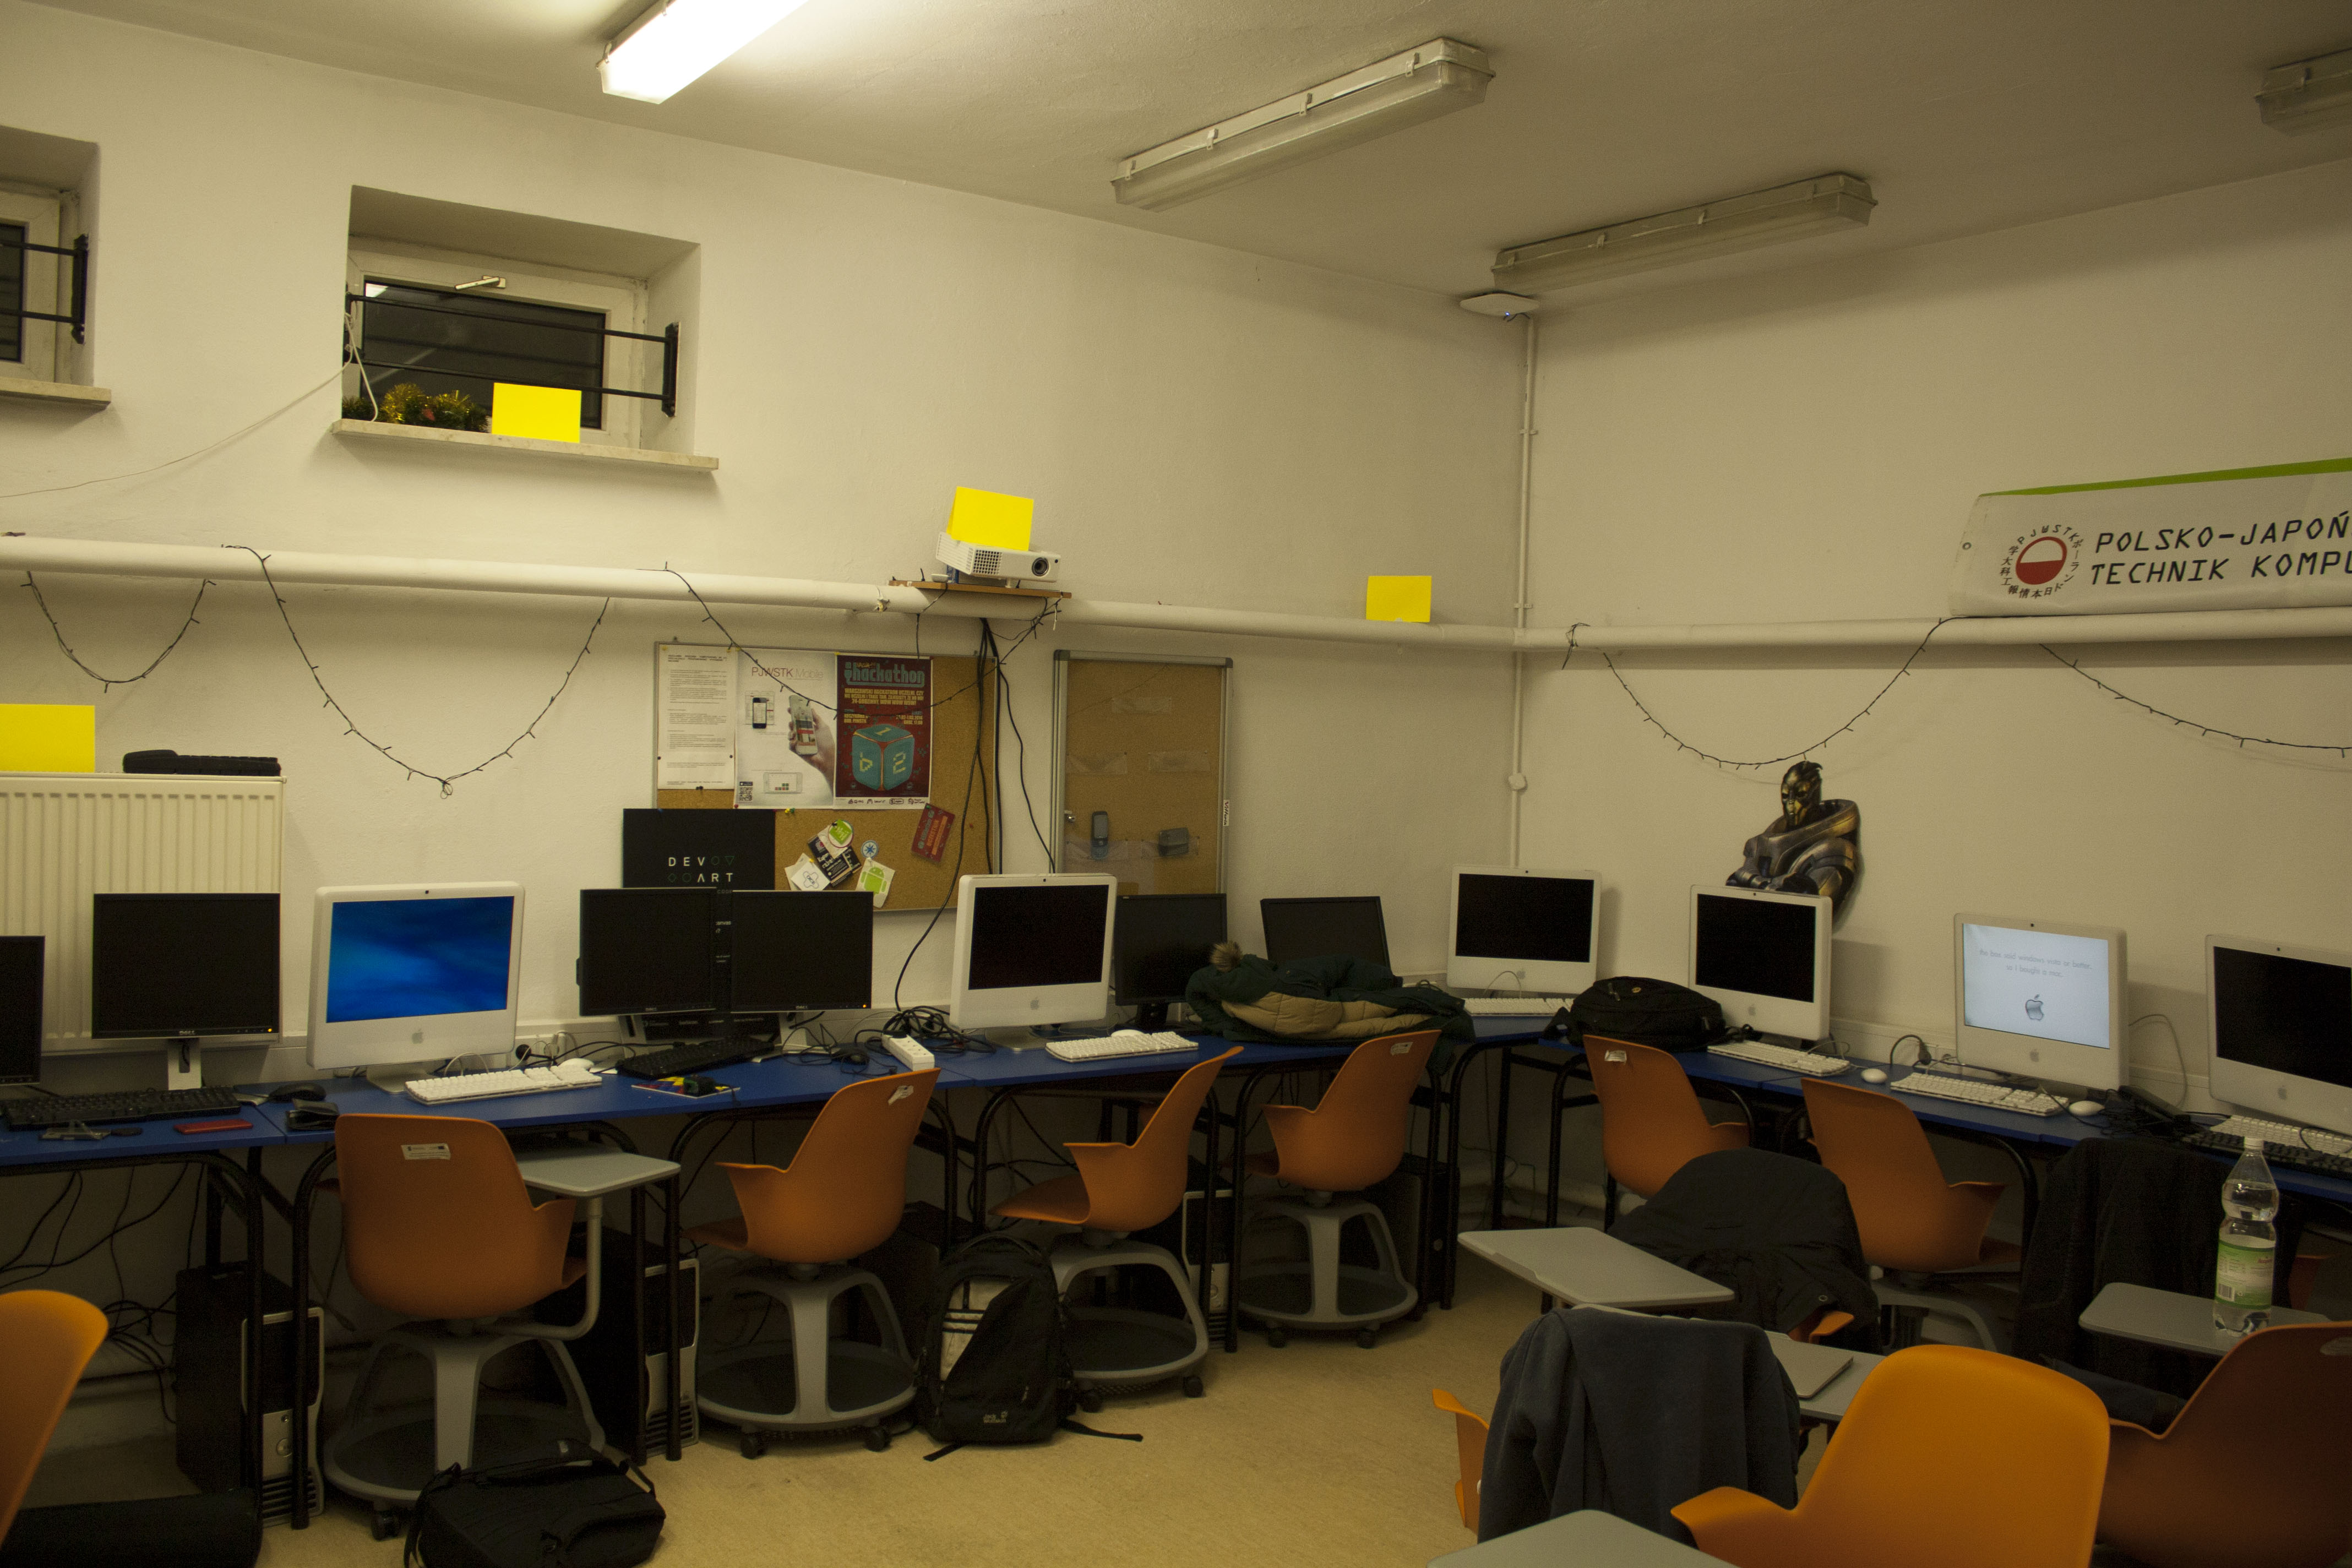
\includegraphics[width=0.9\textwidth]{images/s9.jpg}
\captionof{figure}{
Labolatorium PJATK
}
\small {źródło własne }
\end{center}

\paragraph{}
Głównym założeniem było stworzenie minigry opartej na grze z początku lat dziewiędziesiątych o nazwie Lemmingi \footnote{https://en.wikipedia.org/wiki/Lemmings}. Pierwotnie gra została stworzona w 1991 roku na platformę Amiga.

Celem gry jest doprowadzenie grupy aktorów (tytułowych Lemmingów) do wyjścia (mety). Aktorzy automatycznie idą w jedną stronę. Każdemu z nich można włączyć jedną lub więcej umiejętność (np. umiejętność kopania, swobodnego spadania - spadochron). Aktorzy generowani są automatycznie w określonej sekwencji czasu.

\subsection{Implementacja w technologii hologramu}
\paragraph{}
Pierwotnym założeniem było stworzenie projektu za pomocą hologramu. Planowano wykorzystanie złudzenia optycznego stworzonego za pomocą światła na półprzezroczystej płaszczyźnie znajdującej się przed oczami odbiorcy. Analogiczną koncepcję prezentowało w przeszłości urządzenie Google Glass, a obecnie np. Microsoft Hololens lub Meta2.

Jednakże zamiast urządzenia nakładanego na głowę planowano użyć przezroczystą szybę znajdującą się na drzwiach wejściowych do labolatorium. Dzięki takiem rozwiązaniu odbiór instalacji odbywałby się bez dodatkowych urządzeń, co za tym idzie interakcja byłaby bardziej naturalna.
Na szybie umieszczona zostałaby warstwa półprzezroczystej folii na której prezentowany byłby obraz za pomocą projektora multimedialnego ustawionego pod kątem około 30 stopni w górę w kierunku szyby. Projektor znajdowałby się na statywie w środu sali - technologia projekcja tylna.

Podczas eksperymentów próbowano wiele różnych folii oraz kilka ustawień projektorów. 

Zaobserowano:
\begin{itemize}
	\item Umiejscowienie projektora pod kątem względem szyby powoduje bardziej naturalny obraz. Nie widać wtedy głównego strumienia światła z projektora (strumień światła nie jest prowadzony w linii prostej do odbiorcy), co za tym idzie  nie ma odczucia oślepienia.
    \item Użycie specjalnej folii do projekcji tylnej powoduje najlepszy odbiór. Inne folie przepuszczały zbyt małą ilość światła, bądź obraz z projektora był mało ostry.
    \item Użycie projektora w technologii LED okazało się lepsze, niż zastosowanie standardowego projektora multimedialnego. Mała odległość pomiędzy drzwiam, a urządzeniem pozwalała na użycie projektora z małą ilościa lumenów.
\end{itemize}

\paragraph{}
Jednakże zrezygnowano z powyższego pomysłu, ponieważ napotkano problem nakładania obrazu z  elementami znajdującymi się w sali. Aby punkty wirtualne z ich rzeczywistami odpowiednikami się nakładały i tworzyły spójny obraz (augumented reality) należałoby spoglądać przez szybę pod jednym wskazanym kątem. Co za tym idzie prawidłowy odbiór instalacji byłby zaburzony przez takie czynniki jak np. wzrost odbiorcy, kierunek wzroku czy też odległość od szyby. Urządzenia takie jak Microsoft Hololens niwelują ten problem poprzez stałe umiejscowienie półprzezroczystego ekranu w małej odległości od oka. 

\begin{center}
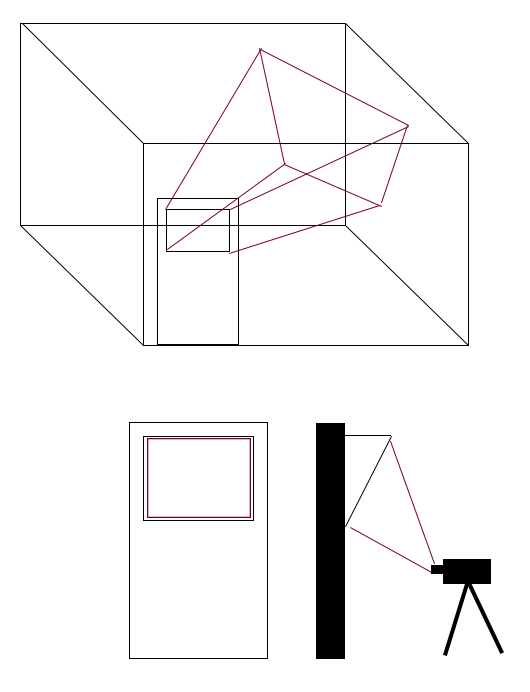
\includegraphics[width=0.9\textwidth]{images/hologramv1.png}
\captionof{figure}{
Poglądowy schemat działania hologramu
}
\small {źródło: własne }
\end{center}

\subsection{Implementacja w technologii mappingu 3d}
\paragraph{}
Kolejnym pomysłem było zastosowanie video mappingu 3d. Jest to technologia często spotykana w branży rozrywkowej (jako tło sceny koncertowej) oraz do prezentowania przestrzeni architektonicznych (zarówno wewnętrznych jak i wewnętrznych), czy też pojazdów jak i innych mniejszych przedmiotów. 
\paragraph{}
Technologia polega na ośwetlaniu rzeczywistego elementu  źródłem światła z projektora multimedialnego. Najlepsze efekty można uzyskać w zaciemnionych pomieszczeniach oraz przy lampach z dużą ilością lumenów. Dzięki temu za pomocą kolorów można pokazywać lub uniewidaczniać elementy przy wykorzystaniu koloru czarnego. Podczas projekcji ciemnego koloru ilość światła z projektora jest bardzo znikoma, co za tym idzie powstaje złudzenie, że element oświetlony światłem czarnym jest niewidoczny.
Przy realizacji większości instalacji takiego typu stosowany jest wcześniej przygotowany obraz wideo. Instalacje nie są interaktywne. Jednakże dzięki temu nawet zaawanowane animacje trójwymiarowe obciążają sprzęt komputerowy tylko podczas renderowania (zamiany obiektów trójwymiarowych na strumień video). Wprowadzenie elementów interaktywnych (np. sterowanie grą) mocno obicąża kartę graficzną komputera.
\paragraph{}
Założono, że projekcja odbywać będzie się na dwóch prostopadłych do siebie ścianach. Takie podejście wymaga dwóch projektorów. Jednakże obraz z nich musi być syncrhonizowany, ponieważ elementy interaktywne (np. postacie) będą przemieszczały się z jednej sciany na drugą. Zastosowanie dwóch komputerów wymagałoby stworzenia protokołu komunikacyjnego. Założono, iż zastosowany będzie jeden komputer z wydajną kartą graficzną, która obsłuży dwa źródła wyjścia.

\begin{center}
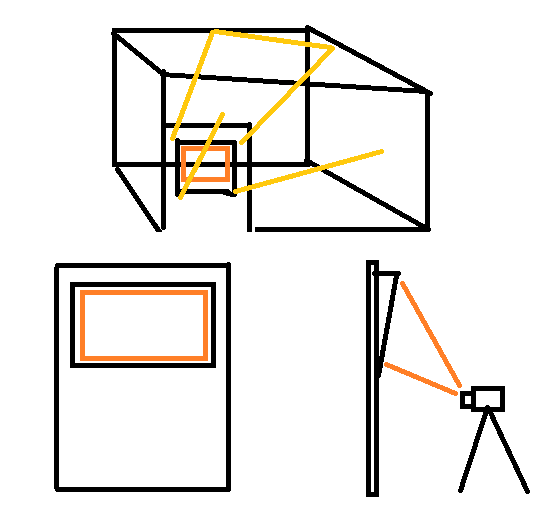
\includegraphics[width=0.9\textwidth]{images/mappingv1.png}
\captionof{figure}{
Poglądowy schemat działania - mapping
}
\small {źródło: własne }
\end{center}

\paragraph{}
Zaobserowano:
\begin{itemize}
	\item Efekty wizualne są odpowiednie, jednakże zauważalny jest brak głębi obrazu. Wszystkie elementy są dwuwymiarowe.
	\item Bardo ważnym aspektem jest jakoś lampy projektora i jego umiejscowienie. Nawet drobne przesunięcie projektora w stosunku do ściany moźe zaburzyć odbiór instalacji.
\end{itemize}
